\documentclass[1p]{elsarticle_modified}
%\bibliographystyle{elsarticle-num}

%\usepackage[colorlinks]{hyperref}
%\usepackage{abbrmath_seonhwa} %\Abb, \Ascr, \Acal ,\Abf, \Afrak
\usepackage{amsfonts}
\usepackage{amssymb}
\usepackage{amsmath}
\usepackage{amsthm}
\usepackage{scalefnt}
\usepackage{amsbsy}
\usepackage{kotex}
\usepackage{caption}
\usepackage{subfig}
\usepackage{color}
\usepackage{graphicx}
\usepackage{xcolor} %% white, black, red, green, blue, cyan, magenta, yellow
\usepackage{float}
\usepackage{setspace}
\usepackage{hyperref}

\usepackage{tikz}
\usetikzlibrary{arrows}

\usepackage{multirow}
\usepackage{array} % fixed length table
\usepackage{hhline}

%%%%%%%%%%%%%%%%%%%%%
\makeatletter
\renewcommand*\env@matrix[1][\arraystretch]{%
	\edef\arraystretch{#1}%
	\hskip -\arraycolsep
	\let\@ifnextchar\new@ifnextchar
	\array{*\c@MaxMatrixCols c}}
\makeatother %https://tex.stackexchange.com/questions/14071/how-can-i-increase-the-line-spacing-in-a-matrix
%%%%%%%%%%%%%%%

\usepackage[normalem]{ulem}

\newcommand{\msout}[1]{\ifmmode\text{\sout{\ensuremath{#1}}}\else\sout{#1}\fi}
%SOURCE: \msout is \stkout macro in https://tex.stackexchange.com/questions/20609/strikeout-in-math-mode

\newcommand{\cancel}[1]{
	\ifmmode
	{\color{red}\msout{#1}}
	\else
	{\color{red}\sout{#1}}
	\fi
}

\newcommand{\add}[1]{
	{\color{blue}\uwave{#1}}
}

\newcommand{\replace}[2]{
	\ifmmode
	{\color{red}\msout{#1}}{\color{blue}\uwave{#2}}
	\else
	{\color{red}\sout{#1}}{\color{blue}\uwave{#2}}
	\fi
}

\newcommand{\Sol}{\mathcal{S}} %segment
\newcommand{\D}{D} %diagram
\newcommand{\A}{\mathcal{A}} %arc


%%%%%%%%%%%%%%%%%%%%%%%%%%%%%5 test

\def\sl{\operatorname{\textup{SL}}(2,\Cbb)}
\def\psl{\operatorname{\textup{PSL}}(2,\Cbb)}
\def\quan{\mkern 1mu \triangleright \mkern 1mu}

\theoremstyle{definition}
\newtheorem{thm}{Theorem}[section]
\newtheorem{prop}[thm]{Proposition}
\newtheorem{lem}[thm]{Lemma}
\newtheorem{ques}[thm]{Question}
\newtheorem{cor}[thm]{Corollary}
\newtheorem{defn}[thm]{Definition}
\newtheorem{exam}[thm]{Example}
\newtheorem{rmk}[thm]{Remark}
\newtheorem{alg}[thm]{Algorithm}

\newcommand{\I}{\sqrt{-1}}
\begin{document}

%\begin{frontmatter}
%
%\title{Boundary parabolic representations of knots up to 8 crossings}
%
%%% Group authors per affiliation:
%\author{Yunhi Cho} 
%\address{Department of Mathematics, University of Seoul, Seoul, Korea}
%\ead{yhcho@uos.ac.kr}
%
%
%\author{Seonhwa Kim} %\fnref{s_kim}}
%\address{Center for Geometry and Physics, Institute for Basic Science, Pohang, 37673, Korea}
%\ead{ryeona17@ibs.re.kr}
%
%\author{Hyuk Kim}
%\address{Department of Mathematical Sciences, Seoul National University, Seoul 08826, Korea}
%\ead{hyukkim@snu.ac.kr}
%
%\author{Seokbeom Yoon}
%\address{Department of Mathematical Sciences, Seoul National University, Seoul, 08826,  Korea}
%\ead{sbyoon15@snu.ac.kr}
%
%\begin{abstract}
%We find all boundary parabolic representation of knots up to 8 crossings.
%
%\end{abstract}
%\begin{keyword}
%    \MSC[2010] 57M25 
%\end{keyword}
%
%\end{frontmatter}

%\linenumbers
%\tableofcontents
%
\newcommand\colored[1]{\textcolor{white}{\rule[-0.35ex]{0.8em}{1.4ex}}\kern-0.8em\color{red} #1}%
%\newcommand\colored[1]{\textcolor{white}{ #1}\kern-2.17ex	\textcolor{white}{ #1}\kern-1.81ex	\textcolor{white}{ #1}\kern-2.15ex\color{red}#1	}

{\Large $\underline{12a_{0204}~(K12a_{0204})}$}

\setlength{\tabcolsep}{10pt}
\renewcommand{\arraystretch}{1.6}
\vspace{1cm}\begin{tabular}{m{100pt}>{\centering\arraybackslash}m{274pt}}
\multirow{5}{120pt}{
	\centering
	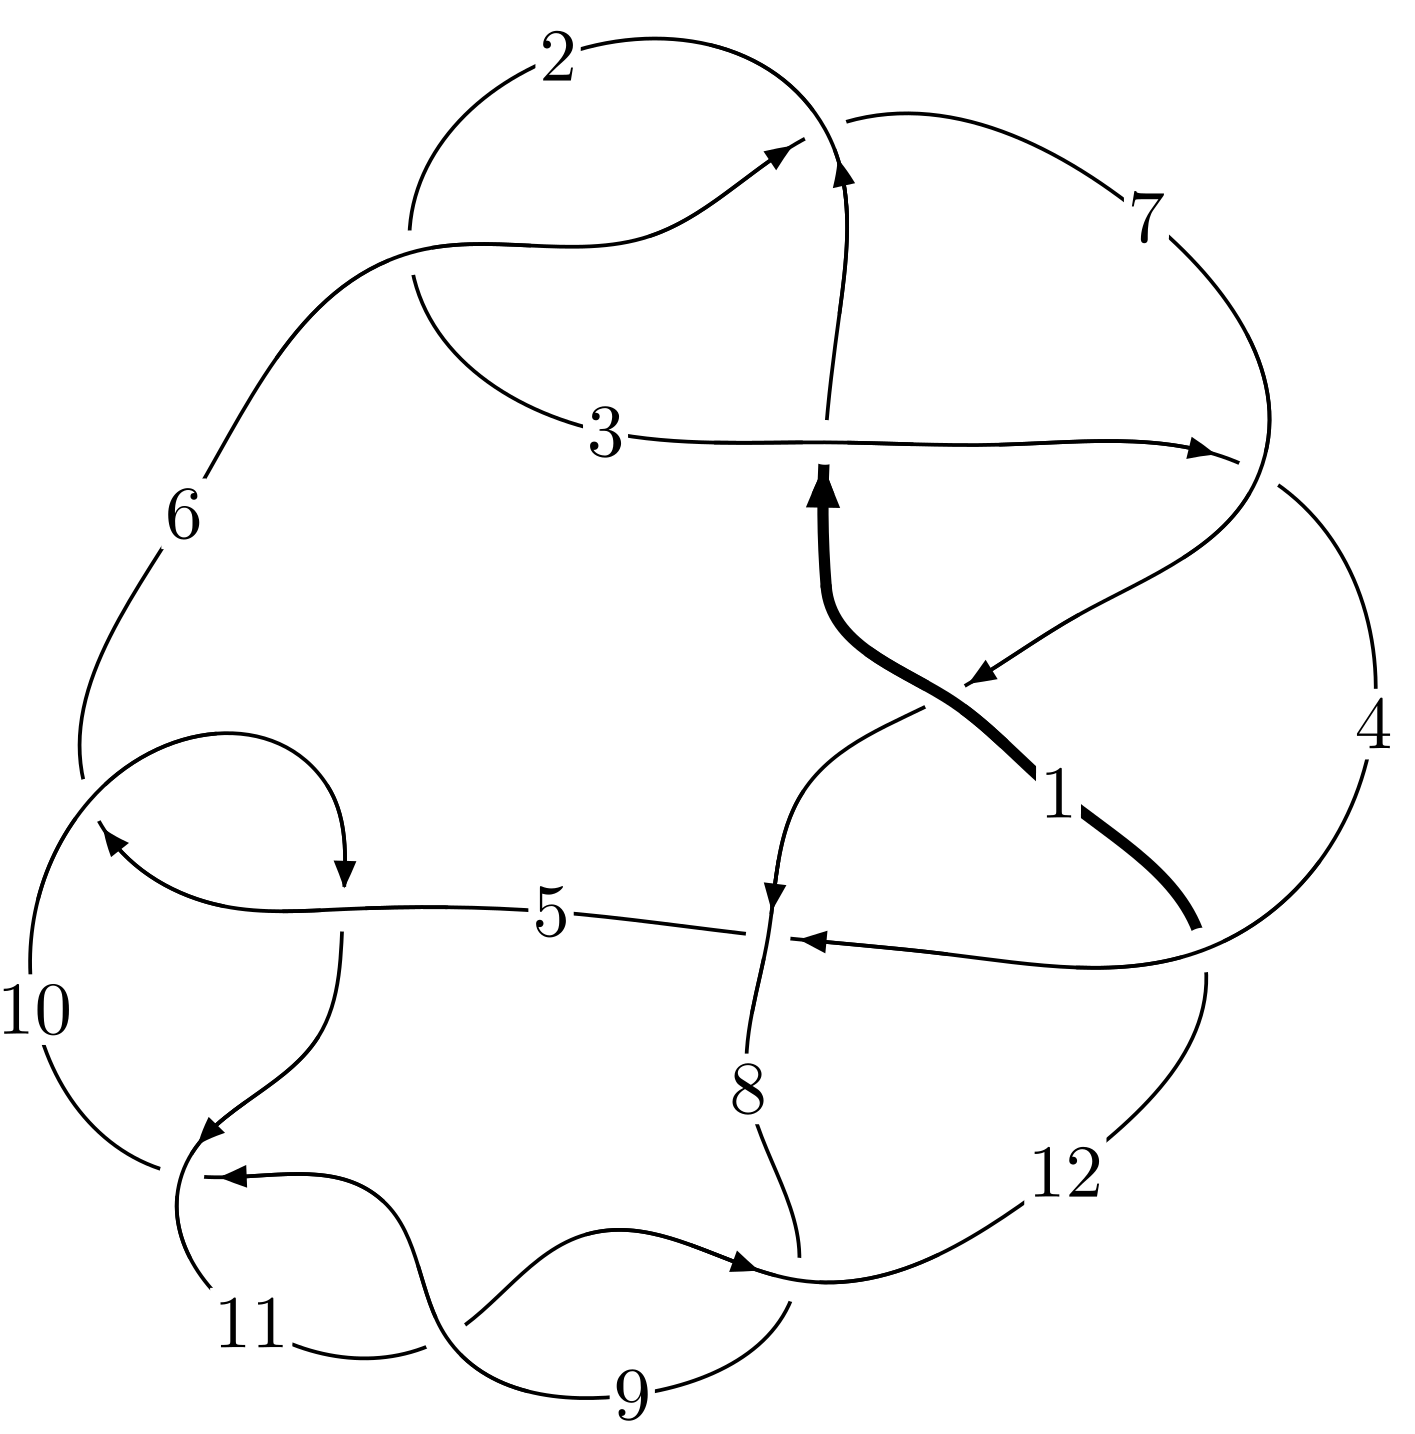
\includegraphics[width=112pt]{../../../GIT/diagram.site/Diagrams/png/1005_12a_0204.png}\\
\ \ \ A knot diagram\footnotemark}&
\allowdisplaybreaks
\textbf{Linearized knot diagam} \\
\cline{2-2}
 &
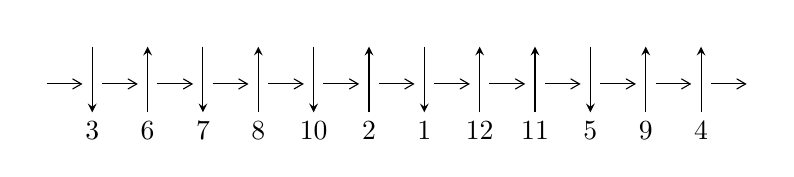
\begin{tikzpicture}[x=20pt, y=17pt]
	% nodes
	\node (C0) at (0, 0) {};
	\node (C1) at (1, 0) {};
	\node (C1U) at (1, +1) {};
	\node (C1D) at (1, -1) {3};

	\node (C2) at (2, 0) {};
	\node (C2U) at (2, +1) {};
	\node (C2D) at (2, -1) {6};

	\node (C3) at (3, 0) {};
	\node (C3U) at (3, +1) {};
	\node (C3D) at (3, -1) {7};

	\node (C4) at (4, 0) {};
	\node (C4U) at (4, +1) {};
	\node (C4D) at (4, -1) {8};

	\node (C5) at (5, 0) {};
	\node (C5U) at (5, +1) {};
	\node (C5D) at (5, -1) {10};

	\node (C6) at (6, 0) {};
	\node (C6U) at (6, +1) {};
	\node (C6D) at (6, -1) {2};

	\node (C7) at (7, 0) {};
	\node (C7U) at (7, +1) {};
	\node (C7D) at (7, -1) {1};

	\node (C8) at (8, 0) {};
	\node (C8U) at (8, +1) {};
	\node (C8D) at (8, -1) {12};

	\node (C9) at (9, 0) {};
	\node (C9U) at (9, +1) {};
	\node (C9D) at (9, -1) {11};

	\node (C10) at (10, 0) {};
	\node (C10U) at (10, +1) {};
	\node (C10D) at (10, -1) {5};

	\node (C11) at (11, 0) {};
	\node (C11U) at (11, +1) {};
	\node (C11D) at (11, -1) {9};

	\node (C12) at (12, 0) {};
	\node (C12U) at (12, +1) {};
	\node (C12D) at (12, -1) {4};
	\node (C13) at (13, 0) {};

	% arrows
	\draw[->,>={angle 60}]
	(C0) edge (C1) (C1) edge (C2) (C2) edge (C3) (C3) edge (C4) (C4) edge (C5) (C5) edge (C6) (C6) edge (C7) (C7) edge (C8) (C8) edge (C9) (C9) edge (C10) (C10) edge (C11) (C11) edge (C12) (C12) edge (C13) ;	\draw[->,>=stealth]
	(C1U) edge (C1D) (C2D) edge (C2U) (C3U) edge (C3D) (C4D) edge (C4U) (C5U) edge (C5D) (C6D) edge (C6U) (C7U) edge (C7D) (C8D) edge (C8U) (C9D) edge (C9U) (C10U) edge (C10D) (C11D) edge (C11U) (C12D) edge (C12U) ;
	\end{tikzpicture} \\
\hhline{~~} \\& 
\textbf{Solving Sequence} \\ \cline{2-2} 
 &
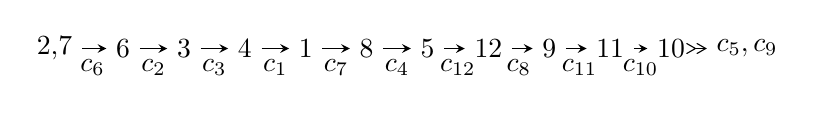
\begin{tikzpicture}[x=22pt, y=7pt]
	% node
	\node (A0) at (-1/8, 0) {2,7};
	\node (A1) at (1, 0) {6};
	\node (A2) at (2, 0) {3};
	\node (A3) at (3, 0) {4};
	\node (A4) at (4, 0) {1};
	\node (A5) at (5, 0) {8};
	\node (A6) at (6, 0) {5};
	\node (A7) at (7, 0) {12};
	\node (A8) at (8, 0) {9};
	\node (A9) at (9, 0) {11};
	\node (A10) at (10, 0) {10};
	\node (C1) at (1/2, -1) {$c_{6}$};
	\node (C2) at (3/2, -1) {$c_{2}$};
	\node (C3) at (5/2, -1) {$c_{3}$};
	\node (C4) at (7/2, -1) {$c_{1}$};
	\node (C5) at (9/2, -1) {$c_{7}$};
	\node (C6) at (11/2, -1) {$c_{4}$};
	\node (C7) at (13/2, -1) {$c_{12}$};
	\node (C8) at (15/2, -1) {$c_{8}$};
	\node (C9) at (17/2, -1) {$c_{11}$};
	\node (C10) at (19/2, -1) {$c_{10}$};
	\node (A11) at (45/4, 0) {$c_{5},c_{9}$};

	% edge
	\draw[->,>=stealth]	
	(A0) edge (A1) (A1) edge (A2) (A2) edge (A3) (A3) edge (A4) (A4) edge (A5) (A5) edge (A6) (A6) edge (A7) (A7) edge (A8) (A8) edge (A9) (A9) edge (A10) ;
	\draw[->>,>={angle 60}]	
	(A10) edge (A11);
\end{tikzpicture} \\ 

\end{tabular} \\

\footnotetext{
The image of knot diagram is generated by the software ``\textbf{Draw programme}" developed by Andrew Bartholomew(\url{http://www.layer8.co.uk/maths/draw/index.htm\#Running-draw}), where we modified some parts for our purpose(\url{https://github.com/CATsTAILs/LinksPainter}).
}\phantom \\ \newline 
\centering \textbf{Ideals for irreducible components\footnotemark of $X_{\text{par}}$} 
 
\begin{align*}
I^u_{1}&=\langle 
u^{86}+u^{85}+\cdots+3 u+1\rangle \\
\\
\end{align*}
\raggedright * 1 irreducible components of $\dim_{\mathbb{C}}=0$, with total 86 representations.\\
\footnotetext{All coefficients of polynomials are rational numbers. But the coefficients are sometimes approximated in decimal forms when there is not enough margin.}
\newpage
\renewcommand{\arraystretch}{1}
\centering \section*{I. $I^u_{1}= \langle u^{86}+u^{85}+\cdots+3 u+1 \rangle$}
\flushleft \textbf{(i) Arc colorings}\\
\begin{tabular}{m{7pt} m{180pt} m{7pt} m{180pt} }
\flushright $a_{2}=$&$\begin{pmatrix}0\\u\end{pmatrix}$ \\
\flushright $a_{7}=$&$\begin{pmatrix}1\\0\end{pmatrix}$ \\
\flushright $a_{6}=$&$\begin{pmatrix}1\\u^2\end{pmatrix}$ \\
\flushright $a_{3}=$&$\begin{pmatrix}u\\u^3+u\end{pmatrix}$ \\
\flushright $a_{4}=$&$\begin{pmatrix}- u^3\\u^3+u\end{pmatrix}$ \\
\flushright $a_{1}=$&$\begin{pmatrix}u^3\\u^5+u^3+u\end{pmatrix}$ \\
\flushright $a_{8}=$&$\begin{pmatrix}u^8+u^6+u^4+1\\u^{10}+2 u^8+3 u^6+2 u^4+u^2\end{pmatrix}$ \\
\flushright $a_{5}=$&$\begin{pmatrix}u^{21}+4 u^{19}+9 u^{17}+12 u^{15}+12 u^{13}+10 u^{11}+9 u^9+6 u^7+3 u^5+u\\u^{23}+5 u^{21}+\cdots+2 u^3+u\end{pmatrix}$ \\
\flushright $a_{12}=$&$\begin{pmatrix}- u^{11}-2 u^9-2 u^7+u^3\\u^{11}+3 u^9+4 u^7+3 u^5+u^3+u\end{pmatrix}$ \\
\flushright $a_{9}=$&$\begin{pmatrix}u^{32}+7 u^{30}+\cdots+2 u^{12}+1\\- u^{32}-8 u^{30}+\cdots-12 u^8-4 u^6\end{pmatrix}$ \\
\flushright $a_{11}=$&$\begin{pmatrix}- u^{53}-12 u^{51}+\cdots-3 u^5- u\\u^{53}+13 u^{51}+\cdots+u^3+u\end{pmatrix}$ \\
\flushright $a_{10}=$&$\begin{pmatrix}u^{74}+17 u^{72}+\cdots+u^2+1\\- u^{74}-18 u^{72}+\cdots-2 u^4- u^2\end{pmatrix}$\\&\end{tabular}
\flushleft \textbf{(ii) Obstruction class $= -1$}\\~\\
\flushleft \textbf{(iii) Cusp Shapes $= 4 u^{85}+4 u^{84}+\cdots+24 u+10$}\\~\\
\newpage\renewcommand{\arraystretch}{1}
\flushleft \textbf{(iv) u-Polynomials at the component}\newline \\
\begin{tabular}{m{50pt}|m{274pt}}
Crossings & \hspace{64pt}u-Polynomials at each crossing \\
\hline $$\begin{aligned}c_{1}\end{aligned}$$&$\begin{aligned}
&u^{86}+41 u^{85}+\cdots+3 u+1
\end{aligned}$\\
\hline $$\begin{aligned}c_{2},c_{6}\end{aligned}$$&$\begin{aligned}
&u^{86}- u^{85}+\cdots-3 u+1
\end{aligned}$\\
\hline $$\begin{aligned}c_{3}\end{aligned}$$&$\begin{aligned}
&u^{86}+u^{85}+\cdots+471 u+65
\end{aligned}$\\
\hline $$\begin{aligned}c_{4}\end{aligned}$$&$\begin{aligned}
&u^{86}- u^{85}+\cdots-149 u+137
\end{aligned}$\\
\hline $$\begin{aligned}c_{5},c_{10}\end{aligned}$$&$\begin{aligned}
&u^{86}- u^{85}+\cdots+u+1
\end{aligned}$\\
\hline $$\begin{aligned}c_{7}\end{aligned}$$&$\begin{aligned}
&u^{86}-5 u^{85}+\cdots-623 u+111
\end{aligned}$\\
\hline $$\begin{aligned}c_{8},c_{9},c_{11}\end{aligned}$$&$\begin{aligned}
&u^{86}-21 u^{85}+\cdots-3 u+1
\end{aligned}$\\
\hline $$\begin{aligned}c_{12}\end{aligned}$$&$\begin{aligned}
&u^{86}+9 u^{85}+\cdots+6433 u+797
\end{aligned}$\\
\hline
\end{tabular}\\~\\
\newpage\renewcommand{\arraystretch}{1}
\flushleft \textbf{(v) Riley Polynomials at the component}\newline \\
\begin{tabular}{m{50pt}|m{274pt}}
Crossings & \hspace{64pt}Riley Polynomials at each crossing \\
\hline $$\begin{aligned}c_{1}\end{aligned}$$&$\begin{aligned}
&y^{86}+9 y^{85}+\cdots+19 y+1
\end{aligned}$\\
\hline $$\begin{aligned}c_{2},c_{6}\end{aligned}$$&$\begin{aligned}
&y^{86}+41 y^{85}+\cdots+3 y+1
\end{aligned}$\\
\hline $$\begin{aligned}c_{3}\end{aligned}$$&$\begin{aligned}
&y^{86}-23 y^{85}+\cdots+399819 y+4225
\end{aligned}$\\
\hline $$\begin{aligned}c_{4}\end{aligned}$$&$\begin{aligned}
&y^{86}+9 y^{85}+\cdots+312079 y+18769
\end{aligned}$\\
\hline $$\begin{aligned}c_{5},c_{10}\end{aligned}$$&$\begin{aligned}
&y^{86}+21 y^{85}+\cdots+3 y+1
\end{aligned}$\\
\hline $$\begin{aligned}c_{7}\end{aligned}$$&$\begin{aligned}
&y^{86}+13 y^{85}+\cdots+865727 y+12321
\end{aligned}$\\
\hline $$\begin{aligned}c_{8},c_{9},c_{11}\end{aligned}$$&$\begin{aligned}
&y^{86}+89 y^{85}+\cdots+11 y+1
\end{aligned}$\\
\hline $$\begin{aligned}c_{12}\end{aligned}$$&$\begin{aligned}
&y^{86}+29 y^{85}+\cdots+40057159 y+635209
\end{aligned}$\\
\hline
\end{tabular}\\~\\
\newpage\flushleft \textbf{(vi) Complex Volumes and Cusp Shapes}
$$\begin{array}{c|c|c}  
\text{Solutions to }I^u_{1}& \I (\text{vol} + \sqrt{-1}CS) & \text{Cusp shape}\\
 \hline 
\begin{aligned}
u &= -0.552073 + 0.903867 I\end{aligned}
 & -4.89234 - 1.96034 I & \phantom{-0.000000 } 0 \\ \hline\begin{aligned}
u &= -0.552073 - 0.903867 I\end{aligned}
 & -4.89234 + 1.96034 I & \phantom{-0.000000 } 0 \\ \hline\begin{aligned}
u &= -0.022062 + 0.940386 I\end{aligned}
 & -5.66854 - 3.02612 I & -3.62148 + 2.70851 I \\ \hline\begin{aligned}
u &= -0.022062 - 0.940386 I\end{aligned}
 & -5.66854 + 3.02612 I & -3.62148 - 2.70851 I \\ \hline\begin{aligned}
u &= \phantom{-}0.561963 + 0.912758 I\end{aligned}
 & -4.52045 - 4.21833 I & \phantom{-0.000000 } 0 \\ \hline\begin{aligned}
u &= \phantom{-}0.561963 - 0.912758 I\end{aligned}
 & -4.52045 + 4.21833 I & \phantom{-0.000000 } 0 \\ \hline\begin{aligned}
u &= \phantom{-}0.642242 + 0.650491 I\end{aligned}
 & -3.74752 + 8.94433 I & \phantom{-}2.00000 - 7.87615 I \\ \hline\begin{aligned}
u &= \phantom{-}0.642242 - 0.650491 I\end{aligned}
 & -3.74752 - 8.94433 I & \phantom{-}2.00000 + 7.87615 I \\ \hline\begin{aligned}
u &= -0.257669 + 1.056490 I\end{aligned}
 & -0.670480 - 0.639201 I & \phantom{-0.000000 } 0 \\ \hline\begin{aligned}
u &= -0.257669 - 1.056490 I\end{aligned}
 & -0.670480 + 0.639201 I & \phantom{-0.000000 } 0 \\ \hline\begin{aligned}
u &= -0.633408 + 0.654906 I\end{aligned}
 & -4.15827 - 2.71284 I & \phantom{-}1.31273 + 3.00115 I \\ \hline\begin{aligned}
u &= -0.633408 - 0.654906 I\end{aligned}
 & -4.15827 + 2.71284 I & \phantom{-}1.31273 - 3.00115 I \\ \hline\begin{aligned}
u &= \phantom{-}0.550086 + 0.961327 I\end{aligned}
 & \phantom{-}2.46470 - 0.37994 I & \phantom{-0.000000 } 0 \\ \hline\begin{aligned}
u &= \phantom{-}0.550086 - 0.961327 I\end{aligned}
 & \phantom{-}2.46470 + 0.37994 I & \phantom{-0.000000 } 0 \\ \hline\begin{aligned}
u &= -0.517375 + 0.987111 I\end{aligned}
 & \phantom{-}0.07166 - 2.62578 I & \phantom{-0.000000 } 0 \\ \hline\begin{aligned}
u &= -0.517375 - 0.987111 I\end{aligned}
 & \phantom{-}0.07166 + 2.62578 I & \phantom{-0.000000 } 0 \\ \hline\begin{aligned}
u &= \phantom{-}0.633756 + 0.606008 I\end{aligned}
 & \phantom{-}3.50780 + 5.03732 I & \phantom{-}7.81344 - 8.08967 I \\ \hline\begin{aligned}
u &= \phantom{-}0.633756 - 0.606008 I\end{aligned}
 & \phantom{-}3.50780 - 5.03732 I & \phantom{-}7.81344 + 8.08967 I \\ \hline\begin{aligned}
u &= -0.238562 + 1.113670 I\end{aligned}
 & -2.23970 + 4.39842 I & \phantom{-0.000000 } 0 \\ \hline\begin{aligned}
u &= -0.238562 - 1.113670 I\end{aligned}
 & -2.23970 - 4.39842 I & \phantom{-0.000000 } 0 \\ \hline\begin{aligned}
u &= \phantom{-}0.264448 + 1.111100 I\end{aligned}
 & -4.27295 - 0.76354 I & \phantom{-0.000000 } 0 \\ \hline\begin{aligned}
u &= \phantom{-}0.264448 - 1.111100 I\end{aligned}
 & -4.27295 + 0.76354 I & \phantom{-0.000000 } 0 \\ \hline\begin{aligned}
u &= \phantom{-}0.554348 + 1.004930 I\end{aligned}
 & \phantom{-}3.01740 + 4.89814 I & \phantom{-0.000000 } 0 \\ \hline\begin{aligned}
u &= \phantom{-}0.554348 - 1.004930 I\end{aligned}
 & \phantom{-}3.01740 - 4.89814 I & \phantom{-0.000000 } 0 \\ \hline\begin{aligned}
u &= \phantom{-}0.311549 + 1.107070 I\end{aligned}
 & -4.74848 + 0.89916 I & \phantom{-0.000000 } 0 \\ \hline\begin{aligned}
u &= \phantom{-}0.311549 - 1.107070 I\end{aligned}
 & -4.74848 - 0.89916 I & \phantom{-0.000000 } 0 \\ \hline\begin{aligned}
u &= -0.347956 + 1.100820 I\end{aligned}
 & -3.34095 - 4.64653 I & \phantom{-0.000000 } 0 \\ \hline\begin{aligned}
u &= -0.347956 - 1.100820 I\end{aligned}
 & -3.34095 + 4.64653 I & \phantom{-0.000000 } 0 \\ \hline\begin{aligned}
u &= \phantom{-}0.635644 + 0.546117 I\end{aligned}
 & \phantom{-}4.36758 - 0.22453 I & \phantom{-}10.66536 + 0.55787 I \\ \hline\begin{aligned}
u &= \phantom{-}0.635644 - 0.546117 I\end{aligned}
 & \phantom{-}4.36758 + 0.22453 I & \phantom{-}10.66536 - 0.55787 I\\
 \hline 
 \end{array}$$\newpage$$\begin{array}{c|c|c}  
\text{Solutions to }I^u_{1}& \I (\text{vol} + \sqrt{-1}CS) & \text{Cusp shape}\\
 \hline 
\begin{aligned}
u &= -0.770174 + 0.323215 I\end{aligned}
 & -5.37084 + 11.03650 I & \phantom{-}0.76608 - 7.01041 I \\ \hline\begin{aligned}
u &= -0.770174 - 0.323215 I\end{aligned}
 & -5.37084 - 11.03650 I & \phantom{-}0.76608 + 7.01041 I \\ \hline\begin{aligned}
u &= -0.588398 + 0.591566 I\end{aligned}
 & \phantom{-}1.23725 - 1.78468 I & \phantom{-}1.82852 + 3.46758 I \\ \hline\begin{aligned}
u &= -0.588398 - 0.591566 I\end{aligned}
 & \phantom{-}1.23725 + 1.78468 I & \phantom{-}1.82852 - 3.46758 I \\ \hline\begin{aligned}
u &= -0.239868 + 1.142870 I\end{aligned}
 & -9.93808 + 8.18745 I & \phantom{-0.000000 } 0 \\ \hline\begin{aligned}
u &= -0.239868 - 1.142870 I\end{aligned}
 & -9.93808 - 8.18745 I & \phantom{-0.000000 } 0 \\ \hline\begin{aligned}
u &= \phantom{-}0.245139 + 1.142850 I\end{aligned}
 & -10.34130 - 1.86383 I & \phantom{-0.000000 } 0 \\ \hline\begin{aligned}
u &= \phantom{-}0.245139 - 1.142850 I\end{aligned}
 & -10.34130 + 1.86383 I & \phantom{-0.000000 } 0 \\ \hline\begin{aligned}
u &= \phantom{-}0.767277 + 0.318425 I\end{aligned}
 & -5.80930 - 4.73542 I & -0.13133 + 2.18376 I \\ \hline\begin{aligned}
u &= \phantom{-}0.767277 - 0.318425 I\end{aligned}
 & -5.80930 + 4.73542 I & -0.13133 - 2.18376 I \\ \hline\begin{aligned}
u &= \phantom{-}0.676444 + 0.477199 I\end{aligned}
 & -1.06723 - 3.95000 I & \phantom{-}4.49030 + 3.18305 I \\ \hline\begin{aligned}
u &= \phantom{-}0.676444 - 0.477199 I\end{aligned}
 & -1.06723 + 3.95000 I & \phantom{-}4.49030 - 3.18305 I \\ \hline\begin{aligned}
u &= -0.748230 + 0.339955 I\end{aligned}
 & \phantom{-}2.22223 + 7.05409 I & \phantom{-}5.75869 - 7.62186 I \\ \hline\begin{aligned}
u &= -0.748230 - 0.339955 I\end{aligned}
 & \phantom{-}2.22223 - 7.05409 I & \phantom{-}5.75869 + 7.62186 I \\ \hline\begin{aligned}
u &= -0.680511 + 0.452157 I\end{aligned}
 & -1.17586 - 1.85794 I & \phantom{-}4.15708 + 2.29378 I \\ \hline\begin{aligned}
u &= -0.680511 - 0.452157 I\end{aligned}
 & -1.17586 + 1.85794 I & \phantom{-}4.15708 - 2.29378 I \\ \hline\begin{aligned}
u &= \phantom{-}0.567898 + 1.043900 I\end{aligned}
 & -2.72701 + 8.77066 I & \phantom{-0.000000 } 0 \\ \hline\begin{aligned}
u &= \phantom{-}0.567898 - 1.043900 I\end{aligned}
 & -2.72701 - 8.77066 I & \phantom{-0.000000 } 0 \\ \hline\begin{aligned}
u &= \phantom{-}0.339044 + 1.142000 I\end{aligned}
 & -11.40330 + 1.33625 I & \phantom{-0.000000 } 0 \\ \hline\begin{aligned}
u &= \phantom{-}0.339044 - 1.142000 I\end{aligned}
 & -11.40330 - 1.33625 I & \phantom{-0.000000 } 0 \\ \hline\begin{aligned}
u &= -0.344970 + 1.141800 I\end{aligned}
 & -11.12770 - 7.68084 I & \phantom{-0.000000 } 0 \\ \hline\begin{aligned}
u &= -0.344970 - 1.141800 I\end{aligned}
 & -11.12770 + 7.68084 I & \phantom{-0.000000 } 0 \\ \hline\begin{aligned}
u &= -0.562524 + 1.055970 I\end{aligned}
 & -2.94385 - 2.95008 I & \phantom{-0.000000 } 0 \\ \hline\begin{aligned}
u &= -0.562524 - 1.055970 I\end{aligned}
 & -2.94385 + 2.95008 I & \phantom{-0.000000 } 0 \\ \hline\begin{aligned}
u &= -0.713316 + 0.364912 I\end{aligned}
 & \phantom{-}3.53763 + 1.70720 I & \phantom{-}9.34373 - 0.47522 I \\ \hline\begin{aligned}
u &= -0.713316 - 0.364912 I\end{aligned}
 & \phantom{-}3.53763 - 1.70720 I & \phantom{-}9.34373 + 0.47522 I \\ \hline\begin{aligned}
u &= \phantom{-}0.727927 + 0.324780 I\end{aligned}
 & \phantom{-}0.00076 - 3.48701 I & -0.10685 + 2.81460 I \\ \hline\begin{aligned}
u &= \phantom{-}0.727927 - 0.324780 I\end{aligned}
 & \phantom{-}0.00076 + 3.48701 I & -0.10685 - 2.81460 I \\ \hline\begin{aligned}
u &= -0.509299 + 1.093680 I\end{aligned}
 & -2.26558 - 2.69665 I & \phantom{-0.000000 } 0 \\ \hline\begin{aligned}
u &= -0.509299 - 1.093680 I\end{aligned}
 & -2.26558 + 2.69665 I & \phantom{-0.000000 } 0\\
 \hline 
 \end{array}$$\newpage$$\begin{array}{c|c|c}  
\text{Solutions to }I^u_{1}& \I (\text{vol} + \sqrt{-1}CS) & \text{Cusp shape}\\
 \hline 
\begin{aligned}
u &= \phantom{-}0.532946 + 1.112480 I\end{aligned}
 & -3.24505 + 6.62506 I & \phantom{-0.000000 } 0 \\ \hline\begin{aligned}
u &= \phantom{-}0.532946 - 1.112480 I\end{aligned}
 & -3.24505 - 6.62506 I & \phantom{-0.000000 } 0 \\ \hline\begin{aligned}
u &= -0.560287 + 1.103940 I\end{aligned}
 & \phantom{-}1.37872 - 6.58460 I & \phantom{-0.000000 } 0 \\ \hline\begin{aligned}
u &= -0.560287 - 1.103940 I\end{aligned}
 & \phantom{-}1.37872 + 6.58460 I & \phantom{-0.000000 } 0 \\ \hline\begin{aligned}
u &= -0.504237 + 1.132970 I\end{aligned}
 & -10.05170 - 0.22011 I & \phantom{-0.000000 } 0 \\ \hline\begin{aligned}
u &= -0.504237 - 1.132970 I\end{aligned}
 & -10.05170 + 0.22011 I & \phantom{-0.000000 } 0 \\ \hline\begin{aligned}
u &= \phantom{-}0.509014 + 1.133500 I\end{aligned}
 & -10.25420 + 6.56885 I & \phantom{-0.000000 } 0 \\ \hline\begin{aligned}
u &= \phantom{-}0.509014 - 1.133500 I\end{aligned}
 & -10.25420 - 6.56885 I & \phantom{-0.000000 } 0 \\ \hline\begin{aligned}
u &= \phantom{-}0.556014 + 1.119300 I\end{aligned}
 & -2.31255 + 8.37360 I & \phantom{-0.000000 } 0 \\ \hline\begin{aligned}
u &= \phantom{-}0.556014 - 1.119300 I\end{aligned}
 & -2.31255 - 8.37360 I & \phantom{-0.000000 } 0 \\ \hline\begin{aligned}
u &= -0.565704 + 1.120250 I\end{aligned}
 & -0.06439 - 12.03000 I & \phantom{-0.000000 } 0 \\ \hline\begin{aligned}
u &= -0.565704 - 1.120250 I\end{aligned}
 & -0.06439 + 12.03000 I & \phantom{-0.000000 } 0 \\ \hline\begin{aligned}
u &= \phantom{-}0.565065 + 1.132160 I\end{aligned}
 & -8.19937 + 9.74957 I & \phantom{-0.000000 } 0 \\ \hline\begin{aligned}
u &= \phantom{-}0.565065 - 1.132160 I\end{aligned}
 & -8.19937 - 9.74957 I & \phantom{-0.000000 } 0 \\ \hline\begin{aligned}
u &= -0.567396 + 1.131720 I\end{aligned}
 & -7.7482 - 16.0682 I & \phantom{-0.000000 } 0 \\ \hline\begin{aligned}
u &= -0.567396 - 1.131720 I\end{aligned}
 & -7.7482 + 16.0682 I & \phantom{-0.000000 } 0 \\ \hline\begin{aligned}
u &= \phantom{-}0.665867 + 0.284233 I\end{aligned}
 & -0.89403 - 1.98382 I & -1.24074 + 3.64496 I \\ \hline\begin{aligned}
u &= \phantom{-}0.665867 - 0.284233 I\end{aligned}
 & -0.89403 + 1.98382 I & -1.24074 - 3.64496 I \\ \hline\begin{aligned}
u &= \phantom{-}0.696778 + 0.188590 I\end{aligned}
 & -7.58004 - 2.02263 I & -2.18699 + 2.22834 I \\ \hline\begin{aligned}
u &= \phantom{-}0.696778 - 0.188590 I\end{aligned}
 & -7.58004 + 2.02263 I & -2.18699 - 2.22834 I \\ \hline\begin{aligned}
u &= -0.692184 + 0.175922 I\end{aligned}
 & -7.35283 - 4.28364 I & -1.74327 + 2.87228 I \\ \hline\begin{aligned}
u &= -0.692184 - 0.175922 I\end{aligned}
 & -7.35283 + 4.28364 I & -1.74327 - 2.87228 I \\ \hline\begin{aligned}
u &= -0.325865 + 0.553283 I\end{aligned}
 & \phantom{-}0.082965 - 1.264650 I & \phantom{-}0.85289 + 5.85230 I \\ \hline\begin{aligned}
u &= -0.325865 - 0.553283 I\end{aligned}
 & \phantom{-}0.082965 + 1.264650 I & \phantom{-}0.85289 - 5.85230 I \\ \hline\begin{aligned}
u &= -0.561379 + 0.192622 I\end{aligned}
 & \phantom{-}0.06888 - 1.56934 I & \phantom{-}2.04853 + 4.27715 I \\ \hline\begin{aligned}
u &= -0.561379 - 0.192622 I\end{aligned}
 & \phantom{-}0.06888 + 1.56934 I & \phantom{-}2.04853 - 4.27715 I\\
 \hline 
 \end{array}$$\newpage
\newpage\renewcommand{\arraystretch}{1}
\centering \section*{ II. u-Polynomials}
\begin{tabular}{m{50pt}|m{274pt}}
Crossings & \hspace{64pt}u-Polynomials at each crossing \\
\hline $$\begin{aligned}c_{1}\end{aligned}$$&$\begin{aligned}
&u^{86}+41 u^{85}+\cdots+3 u+1
\end{aligned}$\\
\hline $$\begin{aligned}c_{2},c_{6}\end{aligned}$$&$\begin{aligned}
&u^{86}- u^{85}+\cdots-3 u+1
\end{aligned}$\\
\hline $$\begin{aligned}c_{3}\end{aligned}$$&$\begin{aligned}
&u^{86}+u^{85}+\cdots+471 u+65
\end{aligned}$\\
\hline $$\begin{aligned}c_{4}\end{aligned}$$&$\begin{aligned}
&u^{86}- u^{85}+\cdots-149 u+137
\end{aligned}$\\
\hline $$\begin{aligned}c_{5},c_{10}\end{aligned}$$&$\begin{aligned}
&u^{86}- u^{85}+\cdots+u+1
\end{aligned}$\\
\hline $$\begin{aligned}c_{7}\end{aligned}$$&$\begin{aligned}
&u^{86}-5 u^{85}+\cdots-623 u+111
\end{aligned}$\\
\hline $$\begin{aligned}c_{8},c_{9},c_{11}\end{aligned}$$&$\begin{aligned}
&u^{86}-21 u^{85}+\cdots-3 u+1
\end{aligned}$\\
\hline $$\begin{aligned}c_{12}\end{aligned}$$&$\begin{aligned}
&u^{86}+9 u^{85}+\cdots+6433 u+797
\end{aligned}$\\
\hline
\end{tabular}\newpage\renewcommand{\arraystretch}{1}
\centering \section*{ III. Riley Polynomials}
\begin{tabular}{m{50pt}|m{274pt}}
Crossings & \hspace{64pt}Riley Polynomials at each crossing \\
\hline $$\begin{aligned}c_{1}\end{aligned}$$&$\begin{aligned}
&y^{86}+9 y^{85}+\cdots+19 y+1
\end{aligned}$\\
\hline $$\begin{aligned}c_{2},c_{6}\end{aligned}$$&$\begin{aligned}
&y^{86}+41 y^{85}+\cdots+3 y+1
\end{aligned}$\\
\hline $$\begin{aligned}c_{3}\end{aligned}$$&$\begin{aligned}
&y^{86}-23 y^{85}+\cdots+399819 y+4225
\end{aligned}$\\
\hline $$\begin{aligned}c_{4}\end{aligned}$$&$\begin{aligned}
&y^{86}+9 y^{85}+\cdots+312079 y+18769
\end{aligned}$\\
\hline $$\begin{aligned}c_{5},c_{10}\end{aligned}$$&$\begin{aligned}
&y^{86}+21 y^{85}+\cdots+3 y+1
\end{aligned}$\\
\hline $$\begin{aligned}c_{7}\end{aligned}$$&$\begin{aligned}
&y^{86}+13 y^{85}+\cdots+865727 y+12321
\end{aligned}$\\
\hline $$\begin{aligned}c_{8},c_{9},c_{11}\end{aligned}$$&$\begin{aligned}
&y^{86}+89 y^{85}+\cdots+11 y+1
\end{aligned}$\\
\hline $$\begin{aligned}c_{12}\end{aligned}$$&$\begin{aligned}
&y^{86}+29 y^{85}+\cdots+40057159 y+635209
\end{aligned}$\\
\hline
\end{tabular}
\vskip 2pc
\end{document}